% =====================================================================
% Snippet: hyperparams-table.tex
% =====================================================================
% USAGE: Multi-row hyperparameter table with right-aligned values.
% Copy tikzpicture content (lines marked %% COPY-START / END), then:
%   - rows: \def\tabdata{key/value, key/value, ...}
%   - origin_x, origin_y: anchor position
%   - title: table title
%   - header_color: title bar color (default acaTealLine)
%   - row_height: cm per row (default 0.4)
%   - col_width: total table width (default 4.0cm)
%
% Supports up to ~10 rows comfortably. For wider data use multi-column
% via parallel \tabdata blocks at offset x.
% =====================================================================

\documentclass[tikz,border=10pt]{standalone}
\usepackage{xcolor,tikz}
\usetikzlibrary{positioning,calc}

\definecolor{acaTealLine}{HTML}{1F8F8F}
\definecolor{acaTealFill}{HTML}{D3EBEB}
\definecolor{acaGreyLine}{HTML}{606060}
\definecolor{acaGreyLight}{HTML}{F0F0F0}

\begin{document}
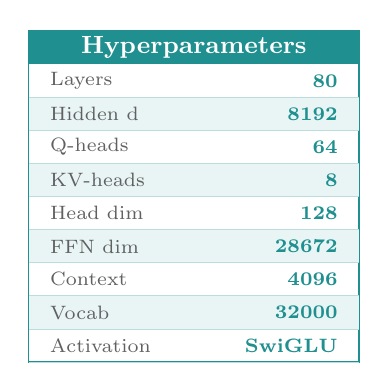
\begin{tikzpicture}

%% COPY-START =========================================================

% --- PARAMETERS ---
\def\tabdata{%
  Layers/80,%
  Hidden d/8192,%
  Q-heads/64,%
  KV-heads/8,%
  Head dim/128,%
  FFN dim/28672,%
  Context/4096,%
  Vocab/32000,%
  Activation/SwiGLU%
}
\def\xO{0}              % origin x
\def\yO{0}              % origin y (top of table)
\def\rowH{0.42}         % row height in cm
\def\colW{4.2}          % total table width in cm
\def\headColor{acaTealLine}
\def\fillColor{acaTealFill}

% --- TITLE BAR ---
\fill[\headColor] (\xO, \yO) rectangle (\xO + \colW, \yO + \rowH);
\node[anchor=center, font=\small\bfseries, color=white]
  at (\xO + \colW/2, \yO + \rowH/2) {Hyperparameters};

% --- TABLE BORDER ---
\newcount\rowcount \rowcount=0
\foreach \k/\v in \tabdata { \global\advance\rowcount by 1 }
\edef\nrows{\the\rowcount}
\pgfmathsetmacro\tabH{\nrows * \rowH}
\draw[\headColor, line width=0.6pt]
  (\xO, \yO - \tabH) rectangle (\xO + \colW, \yO + \rowH);

% --- ROWS (alternating fill for readability) ---
% Use foreach's built-in [count=\idx] — this is the ONLY reliable
% way to accumulate index across iterations. \pgfmathsetmacro\idx{\idx+1}
% can fail silently because foreach has local scope.
\foreach [count=\idx] \k/\v in \tabdata {
  \pgfmathsetmacro\ypos{\yO - (\idx - 1) * \rowH}
  \pgfmathsetmacro\altfill{int(mod(\idx,2))}
  % alternate row fill
  \ifnum\altfill=0
    \fill[\fillColor!50] (\xO, \ypos - \rowH) rectangle (\xO + \colW, \ypos);
  \fi
  % key (left)
  \node[anchor=west, font=\scriptsize, color=acaGreyLine]
    at (\xO + 0.15, \ypos - \rowH/2) {\k};
  % value (right)
  \node[anchor=east, font=\scriptsize\bfseries, color=\headColor]
    at (\xO + \colW - 0.15, \ypos - \rowH/2) {\v};
}

% --- HORIZONTAL DIVIDERS ---
\foreach \i in {1,...,\nrows} {
  \pgfmathsetmacro\ypos{\yO - \i * \rowH}
  \draw[\headColor!30, line width=0.3pt]
    (\xO, \ypos) -- (\xO + \colW, \ypos);
}

%% COPY-END ===========================================================

\end{tikzpicture}
\end{document}
